\documentclass{standalone}
\usepackage{tikz}
\usetikzlibrary{patterns, positioning}

\begin{document}
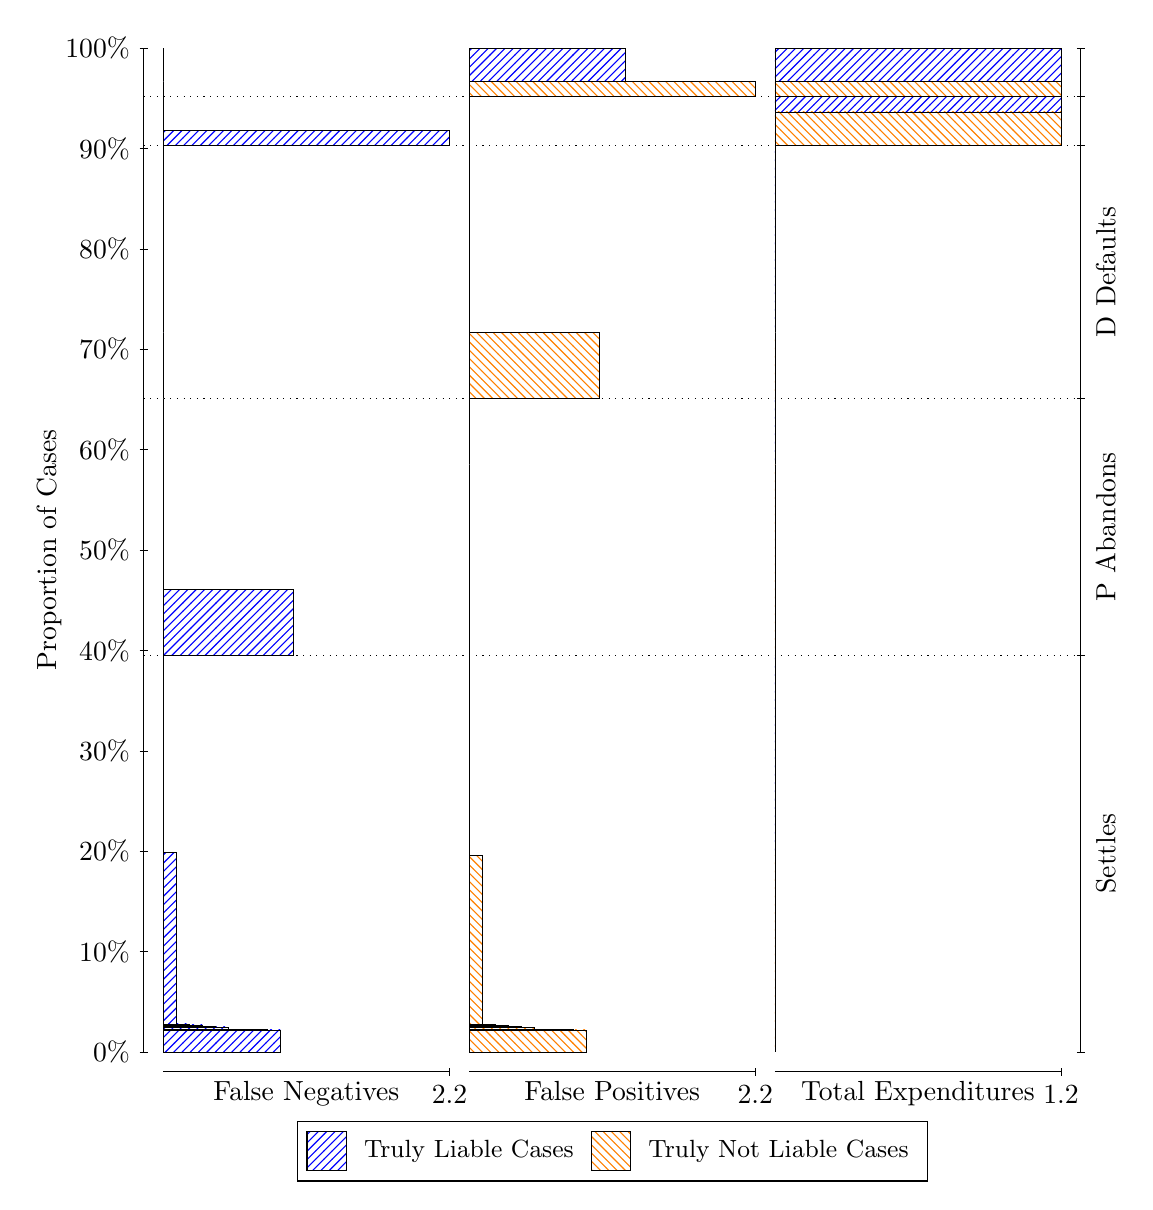
\begin{tikzpicture}
\draw[black, very thin] (1.5,1.75) -- (1.5,14.5);
\node[rotate=90, anchor=center] at (0.3, 8.125) {Proportion of Cases};
\draw[black, very thin] (1.45,1.75) -- (1.55,1.75);
\node[anchor=east] at (1.45, 1.75) {0\%};
\draw[black, very thin] (1.45,3.025) -- (1.55,3.025);
\node[anchor=east] at (1.45, 3.025) {10\%};
\draw[black, very thin] (1.45,4.3) -- (1.55,4.3);
\node[anchor=east] at (1.45, 4.3) {20\%};
\draw[black, very thin] (1.45,5.575) -- (1.55,5.575);
\node[anchor=east] at (1.45, 5.575) {30\%};
\draw[black, very thin] (1.45,6.85) -- (1.55,6.85);
\node[anchor=east] at (1.45, 6.85) {40\%};
\draw[black, very thin] (1.45,8.125) -- (1.55,8.125);
\node[anchor=east] at (1.45, 8.125) {50\%};
\draw[black, very thin] (1.45,9.4) -- (1.55,9.4);
\node[anchor=east] at (1.45, 9.4) {60\%};
\draw[black, very thin] (1.45,10.675) -- (1.55,10.675);
\node[anchor=east] at (1.45, 10.675) {70\%};
\draw[black, very thin] (1.45,11.95) -- (1.55,11.95);
\node[anchor=east] at (1.45, 11.95) {80\%};
\draw[black, very thin] (1.45,13.225) -- (1.55,13.225);
\node[anchor=east] at (1.45, 13.225) {90\%};
\draw[black, very thin] (1.45,14.5) -- (1.55,14.5);
\node[anchor=east] at (1.45, 14.5) {100\%};

\draw[black, very thin] (13.4,1.75) -- (13.4,14.5);
\draw[black, very thin] (13.35,1.75) -- (13.45,1.75);
\node[anchor=west] at (13.35, 1.75) {};
\draw[black, very thin] (13.35,6.789) -- (13.45,6.789);
\node[anchor=west] at (13.35, 6.789) {};
\draw[black, very thin] (13.35,10.052) -- (13.45,10.052);
\node[anchor=west] at (13.35, 10.052) {};
\draw[black, very thin] (13.35,13.263) -- (13.45,13.263);
\node[anchor=west] at (13.35, 13.263) {};
\draw[black, very thin] (13.35,13.881) -- (13.45,13.881);
\node[anchor=west] at (13.35, 13.881) {};
\draw[black, very thin] (13.35,14.5) -- (13.45,14.5);
\node[anchor=west] at (13.35, 14.5) {};

\draw[black, very thin, pattern color=blue, pattern=north east lines] (1.75,1.75) rectangle (3.2364,2.0314);
\draw[black, very thin, pattern color=blue, pattern=north east lines] (1.75,2.0314) rectangle (3.0712,2.0342);
\draw[black, very thin, pattern color=blue, pattern=north east lines] (1.75,2.0342) rectangle (2.9061,2.0374);
\draw[black, very thin, pattern color=blue, pattern=north east lines] (1.75,2.0374) rectangle (2.7409,2.0402);
\draw[black, very thin, pattern color=blue, pattern=north east lines] (1.75,2.0402) rectangle (2.7409,2.0407);
\draw[black, very thin, pattern color=blue, pattern=north east lines] (1.75,2.0407) rectangle (2.5758,2.0674);
\draw[black, very thin, pattern color=blue, pattern=north east lines] (1.75,2.0674) rectangle (2.4106,2.0799);
\draw[black, very thin, pattern color=blue, pattern=north east lines] (1.75,2.0799) rectangle (2.2455,2.0927);
\draw[black, very thin, pattern color=blue, pattern=north east lines] (1.75,2.0927) rectangle (2.0803,2.1054);
\draw[black, very thin, pattern color=blue, pattern=north east lines] (1.75,2.1054) rectangle (1.9152,4.289);
\draw[black, very thin, pattern color=orange, pattern=north west lines] (1.75,4.289) rectangle (1.75,6.789);
\draw[black, very thin, pattern color=blue, pattern=north east lines] (1.75,6.789) rectangle (3.4015,7.6285);
\draw[black, very thin, pattern color=orange, pattern=north west lines] (1.75,7.6285) rectangle (1.75,10.052);
\draw[black, very thin, pattern color=orange, pattern=north west lines] (1.75,10.052) rectangle (1.75,10.886);
\draw[black, very thin, pattern color=blue, pattern=north east lines] (1.75,10.886) rectangle (1.75,13.263);
\draw[black, very thin, pattern color=blue, pattern=north east lines] (1.75,13.263) rectangle (5.3833,13.455);
\draw[black, very thin, pattern color=orange, pattern=north west lines] (1.75,13.455) rectangle (1.75,13.881);
\draw[black, very thin, pattern color=orange, pattern=north west lines] (1.75,13.881) rectangle (1.75,14.073);
\draw[black, very thin, pattern color=blue, pattern=north east lines] (1.75,14.073) rectangle (1.75,14.5);
\draw[black, very thin, pattern color=orange, pattern=north west lines] (5.6333,1.75) rectangle (7.1197,2.0293);
\draw[black, very thin, pattern color=orange, pattern=north west lines] (5.6333,2.0293) rectangle (6.9545,2.0327);
\draw[black, very thin, pattern color=orange, pattern=north west lines] (5.6333,2.0327) rectangle (6.7894,2.0367);
\draw[black, very thin, pattern color=orange, pattern=north west lines] (5.6333,2.0367) rectangle (6.6242,2.0405);
\draw[black, very thin, pattern color=orange, pattern=north west lines] (5.6333,2.0405) rectangle (6.4591,2.0659);
\draw[black, very thin, pattern color=orange, pattern=north west lines] (5.6333,2.0659) rectangle (6.2939,2.0665);
\draw[black, very thin, pattern color=orange, pattern=north west lines] (5.6333,2.0665) rectangle (6.2939,2.0765);
\draw[black, very thin, pattern color=orange, pattern=north west lines] (5.6333,2.0765) rectangle (6.1288,2.0872);
\draw[black, very thin, pattern color=orange, pattern=north west lines] (5.6333,2.0872) rectangle (5.9636,2.0973);
\draw[black, very thin, pattern color=orange, pattern=north west lines] (5.6333,2.0973) rectangle (5.7985,4.25);
\draw[black, very thin, pattern color=blue, pattern=north east lines] (5.6333,4.25) rectangle (5.6333,6.789);
\draw[black, very thin, pattern color=orange, pattern=north west lines] (5.6333,6.789) rectangle (5.6333,9.2123);
\draw[black, very thin, pattern color=blue, pattern=north east lines] (5.6333,9.2123) rectangle (5.6333,10.052);
\draw[black, very thin, pattern color=orange, pattern=north west lines] (5.6333,10.052) rectangle (7.2848,10.886);
\draw[black, very thin, pattern color=blue, pattern=north east lines] (5.6333,10.886) rectangle (5.6333,13.263);
\draw[black, very thin, pattern color=orange, pattern=north west lines] (5.6333,13.263) rectangle (5.6333,13.689);
\draw[black, very thin, pattern color=blue, pattern=north east lines] (5.6333,13.689) rectangle (5.6333,13.881);
\draw[black, very thin, pattern color=orange, pattern=north west lines] (5.6333,13.881) rectangle (9.2667,14.073);
\draw[black, very thin, pattern color=blue, pattern=north east lines] (5.6333,14.073) rectangle (7.6152,14.5);
\draw[black, very thin, pattern color=orange, pattern=north west lines] (9.5167,1.75) rectangle (9.5167,4.25);
\draw[black, very thin, pattern color=blue, pattern=north east lines] (9.5167,4.25) rectangle (9.5167,6.789);
\draw[black, very thin, pattern color=orange, pattern=north west lines] (9.5167,6.789) rectangle (9.5167,9.2123);
\draw[black, very thin, pattern color=blue, pattern=north east lines] (9.5167,9.2123) rectangle (9.5167,10.052);
\draw[black, very thin, pattern color=orange, pattern=north west lines] (9.5167,10.052) rectangle (9.5167,10.886);
\draw[black, very thin, pattern color=blue, pattern=north east lines] (9.5167,10.886) rectangle (9.5167,13.263);
\draw[black, very thin, pattern color=orange, pattern=north west lines] (9.5167,13.263) rectangle (13.15,13.689);
\draw[black, very thin, pattern color=blue, pattern=north east lines] (9.5167,13.689) rectangle (13.15,13.881);
\draw[black, very thin, pattern color=orange, pattern=north west lines] (9.5167,13.881) rectangle (13.15,14.073);
\draw[black, very thin, pattern color=blue, pattern=north east lines] (9.5167,14.073) rectangle (13.15,14.5);
\draw[black, dotted] (1.5,6.789) -- (13.4,6.789);
\draw[black, dotted] (1.5,10.052) -- (13.4,10.052);
\draw[black, dotted] (1.5,13.263) -- (13.4,13.263);
\draw[black, dotted] (1.5,13.881) -- (13.4,13.881);
\draw[black, very thin] (1.75,1.5) -- (5.3833,1.5);
\node[anchor=north] at (3.5667, 1.5) {False Negatives};
\draw[black, very thin] (5.3833,1.45) -- (5.3833,1.55);
\node[anchor=north] at (5.3833, 1.45) {2.2};

\draw[black, very thin] (5.6333,1.5) -- (9.2667,1.5);
\node[anchor=north] at (7.45, 1.5) {False Positives};
\draw[black, very thin] (9.2667,1.45) -- (9.2667,1.55);
\node[anchor=north] at (9.2667, 1.45) {2.2};

\draw[black, very thin] (9.5167,1.5) -- (13.15,1.5);
\node[anchor=north] at (11.333, 1.5) {Total Expenditures};
\draw[black, very thin] (13.15,1.45) -- (13.15,1.55);
\node[anchor=north] at (13.15, 1.45) {1.2};

\node[black, centered, rotate=90] at (13.72, 4.2695) {Settles};
\node[black, centered, rotate=90] at (13.72, 8.4204) {P Abandons};
\node[black, centered, rotate=90] at (13.72, 11.657) {D Defaults};



\draw (7.449999999999999,1.5) node[draw=none] (baseCoordinate) {};
\begin{scope}[align=center]
        \matrix[scale=0.5, draw=black, below=0.5cm of baseCoordinate, nodes={draw}, column sep=0.1cm]{
            \node[rectangle, draw, minimum width=0.5cm, minimum height=0.5cm, pattern=north east lines, pattern color=blue] {}; &
            \node[draw=none, font=\small] (B) {Truly Liable Cases}; &
            \node[rectangle, draw, minimum width=0.5cm, minimum height=0.5cm, pattern=north west lines, pattern color=orange] {}; &
            \node[draw=none, font=\small] (B) {Truly Not Liable Cases}; \\
            };
\end{scope}

\end{tikzpicture}
\end{document}